\section{1174040 - Hagan Rowlenstino A. S}
    \subsection{Teori}
        \subsubsection{Definisi Kecerdasan Buatan}

        Artificial Inteligence atau dapat disebut juga dengan kecerdasan buatan merupakan kecerdasan yang ditambahakn kepada suatu sistem yang dapat diatur dalam konteks ilmiah.Michael Haenlein dan Andreas Kaplan mendefinisikan bahawa AI adalah “kemampuan sebuah sistem untuk menejerjemahkan data eksternal dengan benar, mempelajari data tersebut, dan menggunakannya guna mencapai tujuan dan tugas tertentu melalui adaptasi yang fleksibel”. Kecerdasan ini dibuat dan dimasukkan ke dalam mesin agar dapat melakukan pekerjaan seperti yang dapat dilakukan manusia dengan cepat dan tepat. Bidang- bidang yang menggunakan kecerdasan buatan antara lain logika fuzzy, permainan komputer (games), sistem pakar, jaringan saraf tiruan dan robotika.
        
        \subsubsection{Sejarah Kecerdasan Buatan}
        
        Sejarah kecerdasan buatan ini dimulai dari zaman kuno, mitos ataupun cerita dan desas-desus tentang sebuah mahkluk yang mempunyai kecerdasan serta kesadaran yang diberikan oleh pengrajin. Benih - benih nya mulai ditanam oleh para filsuf klasik yang mencari cara untuk menggambarkan proses berfikir manusia sebagai manipulasi simbol secara mekanis yang memuncah pada penemuan komputer digital di tahun 1940-an, yaitu sebuah mesin yang didasarkan penalaran matematika. Istilah kecerdasan buatan sendiri baru muncul pada tahun 1956, dan teori -teori nya sudah muncul sejak tahun 1941.

        \subsubsection{Perkembangan Kecerdasan Buatan}
        \begin{enumerate}
            \item Perkembangan kecerdasan buatan dimulai dari Era Komputer Elektronik pada tahun 1941. dimana ditemukannya alat penyimpanan dan pemrosesan informasi. Dilanjutkan pada tahun 1949, berhasilnya pembuatan komputer yang mampu menyimpan program yang memunat pekerjaan dalam memasukkan program menjadi lebih mudah.
            \item Masa - masa persiapan AI terjadi pada tahun 1943 - 1956.
            \item Awal Perkembangan AI terjadi pada 1952 - 1969
            \item Perkembagan kecerdasan buatan melambat pada tahun 1966-1974
            \item Sistem Berbasis Pengetahuan pada tahun 1969-1979
            \item ecerdasan Buatan menjadi sebuah industri pada tahun 1980-1988. Kembalinya Jaringan Syaraf tiruan pada tahun 1986-sekarang.
        \end{enumerate}
    \subsection{Instalasi}
        Membuka  https://scikit-learn.org/stable/tutorial/basic/tutorial.html lalu mencobanya.
        \subsubsection{Instalasi library scikit, mencoba kompilasi dan ujicoba contoh kode}
        \begin{enumerate}
            \item Buka anaconda prompt lalu ketikkan "pip install -U scikit-learn" untuk menginstall library scikit
            \begin{figure}[H]
                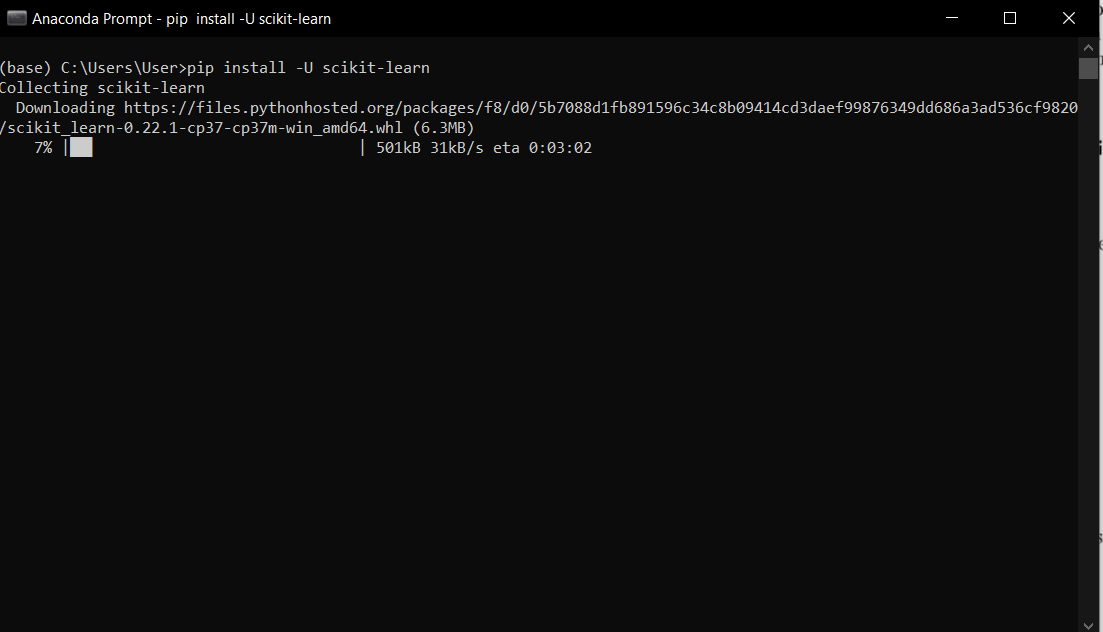
\includegraphics[width=4cm]{figures/1174040/chap1/1.png}
                \centering
                \caption{Install Library Scikit}
            \end{figure}
            \item Pilih salah satu example dari website tersebut lalu jalankan \hfill \break \lstinputlisting[firstline=1]{src/1174040/chap1/ex1.py}
            
            \item buka variable explolernya
            \begin{figure}[H]
                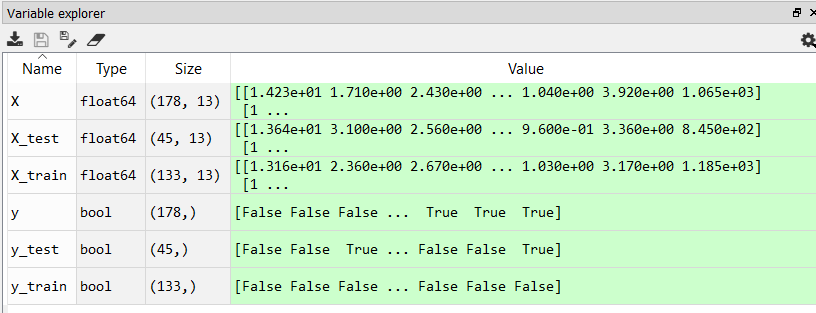
\includegraphics[width=4cm]{figures/1174040/chap1/2.png}
                \centering
                \caption{Variable Exploler}
            \end{figure}
        \end{enumerate}
        \subsubsection{Mencoba loading an example dataset}
        \begin{enumerate}
            \item mengambil data iris dan digit dari dataset \hfill \break \lstinputlisting[firstline=9, lastline=11]{src/1174040/chap1/ex2.py}
            
            \item Menampilkan data digits \hfill \break \lstinputlisting[firstline=13, lastline=13]{src/1174040/chap1/ex2.py}
            
            \begin{figure}[H]
                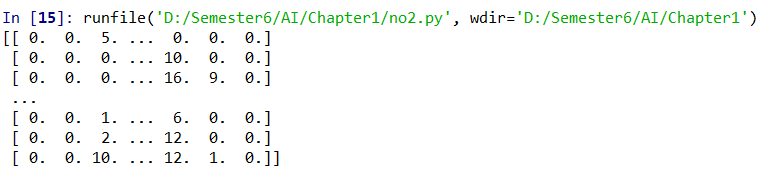
\includegraphics[width=4cm]{figures/1174040/chap1/3.png}
                \centering
                \caption{Data Digits}
            \end{figure}

            \item menampilkan digits.target
            \hfill \break \lstinputlisting[firstline=15, lastline=15]{src/1174040/chap1/ex2.py}

            \begin{figure}[H]
                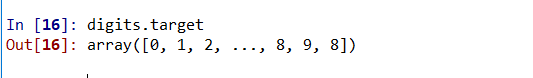
\includegraphics[width=4cm]{figures/1174040/chap1/4.png}
                \centering
                \caption{Digits Target}
            \end{figure}

            \item menampilkan data bentuk 2D. \hfill \break \lstinputlisting[firstline=17, lastline=17]{src/1174040/chap1/ex2.py}

            \begin{figure}[H]
                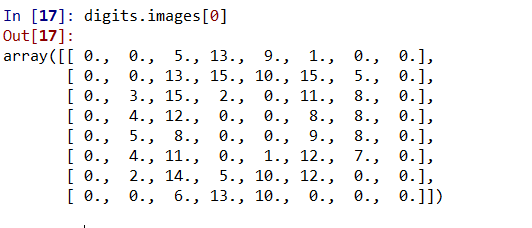
\includegraphics[width=4cm]{figures/1174040/chap1/5.png}
                \centering
                \caption{Data 2D}
            \end{figure}
        \end{enumerate}